% !TEX root = ../vr_st.tex

\section{Barcode estimates}\label{s:computations}

\subsection{$n$-sphere}\label{ss:Sn}

For any integer $n \geq 1$ and real number $r > 0$, let $\bS^n(r)$ be the \defn{$n$-sphere} of radius $r$ centered at the origin of $\R^{n+1}$.
We consider it equipped with the geodesic distance.

\subsubsection{}

Because the Vietoris--Rips complexes of $\bS^n$ is contractible when the scale parameter is greater than $\pi$, all its bars are dominated by $(0, \pi)$.

\subsubsection{} 

Recall from \cite[Thm.~7.1]{lim2020vietoris} that for $n \in \N$ and  $0 < r \leq \zeta_n$, where 
\[\zeta_n \defeq \arccos(\tfrac{-1}{n+1}),\] 
the space $\VR_r(\bS^n)$ is homotopy equivalent to $\bS^n$.
%\anibal{Is this the right citation?}
This implies that, for any degree~$d$, all bars in $\barc\rH_\degp (\VR(\bS^n))$ are dominated by $(\zeta_n,\pi)$ with the exception of a single bar $(0,\zeta_n)$ when $d = n$ (see Figure \ref{fig:Sk}).\footnote{
	The case $n = 1$ has more information.
	From \cite[Thm.~7.4]{adamaszek2017vietoris} it is known that $\VR_r(\bS^1)$ is homotopy equivalent to $\bS^{2n+1}$ for any $n \in \N$ and $\frac{2n\pi}{2n+1} < r \leq \frac{2(n+1)\pi}{2n+3}$.
%	Therefore, for any degree~$d$,
%	\[
%	\barc \rH_{d}(\bS^1) =
%	\begin{cases}
%		\set[\big]{\big(\tfrac{2\ell\pi}{2\ell+1}, \tfrac{2(\ell+1)\pi}{2\ell+3}\big)} & d = 2\ell+1, \\
%		\hfil\emptyset & d = 2\ell.
%	\end{cases}
%	\]
	For $d=1$ and $n > 1$ and one also has more information.
	Recall that a metric space $(\cX, d)$ is said to be a \defn{geodesic space} if for each $x, y \in \cX$ there exists geodesic from $x$ to $y$ of length $d(x, y)$.
	As stated in \cite[Prop.~7.10]{virk20201} one knows that if $\cX$ be a simply-connected geodesic space, then $\barc\rH_1(\cX) = \emptyset$.
	Since the spheres we are considering are geodesic their $\rH_1$ barcode is empty. \ling{We may simplify the footnote.}}
%\anibal{Notice that I am treating the case $n=1$ in here as well since the claims also hold there. I moved the extra information to the footnote.}

\begin{figure}[ht]
	\centering
	\begin{tabular}{ c c }
	\begin{tikzpicture}[scale=0.6]
		\begin{axis} [
			title = {\LARGE $\barc\rH_n(\bS^n)$},
			ticklabel style = {font=\Large},
			axis y line=middle,
			axis x line=middle,
			ytick={0.5,0.57,0.67,0.95},
			yticklabels={,$\zeta_n$,,$\pi$},
			xtick={0.5,0.57,0.95},
			xticklabels={$\frac{\pi}{2}$,$\zeta_n$, $\pi$},
			xmin=-0.015, xmax=1.1,
			ymin=0, ymax=1.1,]
			\addplot [thick,color=black!20!white,fill=black!30!white,
			fill opacity=0.4]coordinates {
				(0.57,0.95)
				(0.57,0.57)
				(0.95,0.95)
				(0.57,0.95)};
			\addplot [black!40!white,mark=none,dashed, thin] coordinates {(0,0.57) (0.57,0.57)};
			\addplot [black!40!white,mark=none,dashed, thin] coordinates {(0.57,0) (0.57,0.57)};
			\addplot[barccolor,mark=*] (0, 0.57) circle (2pt) node[above right,barccolor]{};{\Large\textsf{1}};
			\addplot [mark=none] coordinates {(0,0) (1,1)};
		\end{axis}
	\end{tikzpicture}
	&
	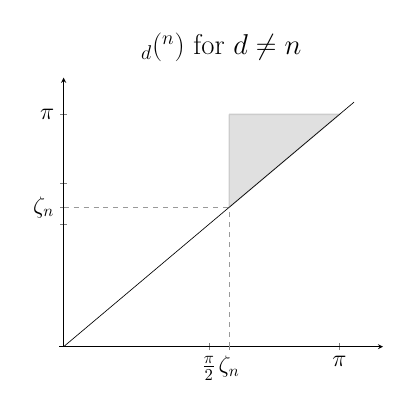
\begin{tikzpicture}[scale=0.6]
		\begin{axis} [
			title = {\LARGE $\barc\rH_d(\bS^n)$ for $d \neq n$},
			ticklabel style = {font=\Large},
			axis y line=middle,
			axis x line=middle,
			ytick={0.5,0.57,0.67,0.95},
			yticklabels={,$\zeta_n$,,$\pi$},
			xtick={0.5,0.57,0.95},
			xticklabels={$\frac{\pi}{2}$,$\zeta_n$, $\pi$},
			xmin=-0.015, xmax=1.1,
			ymin=0, ymax=1.1,]
			\addplot [thick,color=black!20!white,fill=black!30!white,
			fill opacity=0.4]coordinates {
				(0.57,0.95)
				(0.57,0.57)
				(0.95,0.95)
				(0.57,0.95)};
			\addplot [black!40!white,mark=none,dashed, thin] coordinates {(0,0.57) (0.57,0.57)};
			\addplot [black!40!white,mark=none,dashed, thin] coordinates {(0.57,0) (0.57,0.57)};
			\addplot [mark=none] coordinates {(0,0) (1,1)};
		\end{axis}
	\end{tikzpicture}
\end{tabular}
	\caption{Estimation of the persistent homology barcode of $\bS^n$.
		In each figure, the gray area represents the only region, apart from the blue dot, where points could potentially exist within the corresponding barcode.
		Here, and throughout the paper, $\zeta_n = \arccos(\tfrac{-1}{n+1})$ and $\rH_\degp $ denotes reduced $\degp$-homology. \ling{should we mention it is reduced in earlier sections?}
        }
	\label{fig:Sk}
\end{figure}

Similarly, for any linear cohomology operation $\theta \in \cO(\ell,m)$ with $\ell \neq m$, every bar in the barcode of $\img\theta_{\VR(\bS^n)}$ or $\ker\theta_{\VR(\bS^n)}$ is dominated by $(\zeta_n,\pi)$.

%We study the Steenrod barcodes of $\bS^n$.
%For any $k \in \Z_{\geq 1}$, the Steenrod square operation $\Sq^k$ is trivial for $\bS^n$.
%Combined with Proposition \ref{prop:homotopy type} (\ref{prop:Sn}), we conclude that no Steenrod bars can be born before $\zeta_n$.
%Thus, all bars in $\sqbarc{k}{\bS^n}$ are those dominated by $(\zeta_n,\pi)$.

\subsection{Wedge sum of spheres}

The \defn{gluing metric} $d$ on the wedge sum $\bigvee_{i=1}^n \cX_i$ of $n$ metric spaces is defined as follows: for $x \in \cX_i$ and $x' \in \cX_j$ with $i \neq j$,
\[
d(x, x') = d_{\cX_i}(x, x_i) + d_{\cX_j}(x', x_j);
\]
for $x, x' \in \cX_i$, $d(x, x') = d_{\cX_i}(x, x')$.

%and $d_{\cX_1 \vee \cX_2} \vert_{\cX_1 \times \cX_1} = d_{\cX_1},d_{\cX_1 \vee \cX_2} \vert_{\cX_2 \times \cX_2} = d_{\cX_2}$.
%Notice that the above definition can be generalized to the case when we glue $n$ pointed metric spaces $(\cX_1,x_1),\cdots,(\cX_n,x_n)$ by identifying $x_i\sim x_j$ for all $1 \leq i,j\leq n$.
%More generally, the gluing metric on the space $\bigvee_{i=1}^n \cX_i$ is
%\[
%d_{\bigvee_{i=1}^n \cX_i}(x,x') = d_{\cX_i}(x,x_i)+d_{\cX_j}(x',x_j),\forall i\neq j, x \in \cX_i, x' \in \cX_j
%\]
%and $d_{\cX_i \vee \cX_i}|_{\cX_i\times \cX_i} = d_{\cX_i}$ for any $1\leq i\leq n$.

\subsubsection{}\label{prop:wedge sum}
Recall from \cite[Proposition 1 \& Corollary 2]{adamaszek2020homotopy} that the Vietoris--Rips complex of a metric gluing is homotopy equivalent to the wedge sum of the Vietoris--Rips complexes.
From this we deduce that the usual barcode and $\theta$-barcodes of a wedge sum $\cX \vee \cY$ decomposes as the union of the corresponding barcodes of $\cX$ and $\cY$.
%\anibal{Proposition 3.7 doesn't seem to exist in the paper \cite{adamaszek2020homotopy}}

%From this, we deduce the following.
%\facundo{A priory, parameter wise homotopy equivalences do not guarantee same barcodes. One has to have some commutativity. See paper with Osman and Sunhyuk.}
%\ling{I have added the reference}

%\medskip\proposition
%Let $\cX$ and $\cY$ be two compact metric spaces.
%For any degree $d$ we have
%\[
%\rH_\degp (\VR(\cX \vee \cY)) \cong \rH_\degp (\VR(\cX)) \oplus \rH_\degp (\VR(\cY)),
%\]
%and, for any cohomology operation $\theta$, we have
%\begin{align*}
%	\img\theta_{\VR(\cX \vee \cY)} &\cong \img\theta_{\VR(\cX)} \oplus \img\theta_{\VR(\cY)}, \\
%	\ker\theta_{\VR(\cX \vee \cY)} &\cong \ker\theta_{\VR(\cX)} \oplus \ker\theta_{\VR(\cY)}.
%\end{align*}
%\begin{proof}
%	Item (\ref{prop:wedge sum pH}) follows from \cite[Proposition 3.7]{adamaszek2020homotopy} and \cite[Thoerem 6.1 (2)]{lim2020vietoris}.
%	
%	\ling{add the proof of Item (\ref{prop:wedge sum Sq}).}
%\end{proof}

\subsubsection{}

For $n \in \N$ and $\ell_1, \dots, \ell_n \in \N^n$, let
\[
\VS^{\ell_1,\dots,\ell_n} = 
\overbrace{\bS^1\vee\dots\vee\bS^1}^{\ell_1} \vee\dots\vee \overbrace{\bS^n\vee\dots\vee\bS^n}^{\ell_n}.
%(\bS^1)^{\vee m_1} \vee \dots \vee (\bS^n)^{\vee m_n}.
\]
Since $\zeta_{n}$ is decreasing as a function of $n$, the barcode of $\rH_d(\VS^{\ell_1,\dots,\ell_n})$ contains $\ell_d$ copies of $(0,\zeta_d)$ and possibly other bars dominated by $(\zeta_n,\pi)$.
This holds for all degrees with the convention that $\ell_d = 0$ for $d > n$. \ling{double check}

Similarly, for any linear cohomology operation $\theta \in \cO(\ell,m)$ with $\ell \neq m$, every bar in either its $\img\theta$ and $\ker\theta$ barcode is dominated by $(\zeta_n, \pi)$.
\ling{to do: figures need to be adjusted accordingly}
%(top row of Figure \ref{fig:sq barcodes}).

%\proposition For a degree $\degp$, denote $\barc\rH_\degp (\VS^{(\ell_1,\dots,\ell_n)})$ simply as $B_\degp $.
%
%\begin{enumerate}
%	\item $B_1$ is the multiset containing $r_1$ copies of $(0,\tfrac{2\pi}{3})$.
%	\item If $1 < \degp \leq n$, 
%\end{enumerate}
%
%Using Example \ref{ss:Sn} and Proposition \ref{prop:wedge sum} (\ref{prop:wedge sum pH}), we obtain an estimate of the barcodes of $\VS^n$ defined as $\bS^1 \vee \bS^2 \vee \dots \vee \bS^n$, illustrated in the top row of Figure \ref{fig:barcodes}.
%Explicitly, we have the following:
%\begin{itemize}
%	\item $\Hbarc{1}{\VS^n}$ contains only one bar $(0,\tfrac{2\pi}{3})$.
%	\item For any degree $2 \leq m \leq n$, $\Hbarc[\field]{\degp}{\VS^n}$ contains one bar $(0,\zeta_\degp )$, and possibly some bars dominated by $(\zeta_n,\pi)$.
%	For instance, when $m=2l+1$ is odd, $\Hbarc[\field]{\degp}{\VS^n}$ contains the bar $( \tfrac{2l\pi}{2l+1},\tfrac{2(l+1)\pi}{2l+3})$ which is dominated by $(\zeta_n,\pi)$.
%	\item For any degree $\degp > n$, all bars in $\Hbarc[\field]{\degp}{\VS^n}$ are dominated by $(\zeta_n,\pi)$.
%\end{itemize}



%\subsubsection{} Using Example \ref{ss:Sn} and Proposition \ref{prop:wedge sum} (\ref{prop:wedge sum Sq}), we see that all bars in the Steenrod barcodes of $\VS^n$ are dominated by $\cup_{1\leq i\leq n}(\zeta_i,\pi)=(\zeta_n,\pi)$, so they can be illustrated as in the top row of Figure \ref{fig:sq barcodes}.

\begin{figure}
	\centering
	\begin{tikzpicture}[scale=0.52]
	\begin{axis} [
		title = {\LARGE $\Hbarc[\field]{\degp}{\VS^n},1\leq \degp\leq n$},
		ticklabel style = {font=\Large},
		axis y line=middle,
		axis x line=middle,
		ytick={0.5,0.6,0.67,0.95},
		yticklabels={,$\zeta_\degp$,,$\pi$},
		xtick={0.5,0.55,0.95},
		xticklabels={$\frac{\pi}{2}$,$\zeta_n$, $\pi$},
		xmin=-0.015, xmax=1.1,
		ymin=0, ymax=1.1,]
		\addplot [mark=none] coordinates {(0,0) (1,1)};
		\addplot [thick,color=black!20!white,fill=black!30!white,
		fill opacity=0.4]coordinates {
			(0.55,0.95)
			(0.55,0.55)
			(0.95,0.95)
			(0.55,0.95)};
		\addplot [black!40!white,mark=none,dashed, thin] coordinates {(0,0.6) (0.6,0.6)};
		\addplot [black!40!white,mark=none,dashed, thin] coordinates {(0,0.55) (0.55,0.55)};
		\addplot [black!40!white,mark=none,dashed, thin] coordinates {(0.55,0) (0.55,0.55)};
		\addplot[barccolor,mark=*] (0, 0.6) circle (2pt) node[above right,barccolor]{};%{\Large\textsf{1}};
		%\node[mark=none] at (axis cs:0.68,0.21){$\Hbarc{2}{\VS^n}$};
	\end{axis}
\end{tikzpicture}
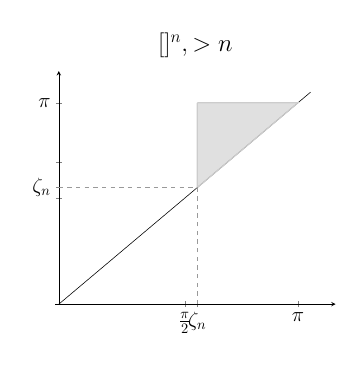
\begin{tikzpicture}[scale=0.52]
	\begin{axis} [
		title = {\LARGE $\Hbarc[\field]{\degp}{\VS^n}, \degp>n$},
		ticklabel style = {font=\Large},
		axis y line=middle,
		axis x line=middle,
		ytick={0.5,0.55,0.67,0.95},
		yticklabels={,$\zeta_n$,,$\pi$},
		xtick={0.5,0.55,0.95},
		xticklabels={$\frac{\pi}{2}$,$\zeta_n$, $\pi$},
		xmin=-0.015, xmax=1.1,
		ymin=0, ymax=1.1,]
		\addplot [mark=none] coordinates {(0,0) (1,1)};
		\addplot [thick,color=black!20!white,fill=black!30!white,
		fill opacity=0.4]coordinates {
			(0.55,0.95)
			(0.55,0.55)
			(0.95,0.95)
			(0.55,0.95)};
		\addplot [black!40!white,mark=none,dashed, thin] coordinates {(0,0.55) (0.55,0.55)};
		\addplot [black!40!white,mark=none,dashed, thin] coordinates {(0.55,0) (0.55,0.55)};
		%\node[mark=none] at (axis cs:0.68,0.21){$\Hbarc[\field]{\degp}{\VS^n}, \degp\geq 3$};
	\end{axis}
\end{tikzpicture}

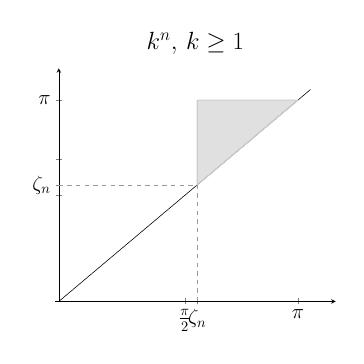
\begin{tikzpicture}[scale=0.52]
	\begin{axis} [
		title={\LARGE $\sqbarc{k}{\VS^n},\, k\geq 1$},
		ticklabel style = {font=\Large},
		axis y line=middle,
		axis x line=middle,
		ytick={0.5,0.55,0.67,0.95},
		yticklabels={,$\zeta_n$,,$\pi$},
		xtick={0.5,0.55,0.95},
		xticklabels={$\frac{\pi}{2}$,$\zeta_n$, $\pi$},
		xmin=-0.015, xmax=1.1,
		ymin=0, ymax=1.1,]
		\addplot [mark=none] coordinates {(0,0) (1,1)};
		\addplot [thick,color=black!20!white,fill=black!30!white,
		fill opacity=0.4]coordinates {
			(0.55,0.95)
			(0.55,0.55)
			(0.95,0.95)
			(0.55,0.95)};
		\addplot [black!40!white,mark=none,dashed, thin] coordinates {(0,0.55) (0.55,0.55)};
		\addplot [black!40!white,mark=none,dashed, thin] coordinates {(0.55,0) (0.55,0.55)};
		%\node[mark=none] at (axis cs:0.68,0.21){$\sqbarc{k}{\VS^n},\, k\geq 1$};
	\end{axis}
\end{tikzpicture}

	\caption{\emph{Top row:} usual barcodes of $\VS^n$. \emph{Bottom row:} Steenrod barcodes of $\VS^n$. \ling{this needs to be adjusted}}
	\label{fig:barcodes}
\end{figure}

\begin{figure}
	\centering
	\begin{tikzpicture}[scale=0.52]
	\begin{axis} [
		title = {\LARGE $\Hbarc{\degp}{\rp^n},\, \degp\leq n$},
		ticklabel style = {font=\Large},
		axis y line=middle,
		axis x line=middle,
		ytick={0.5,0.67,0.95},
		yticklabels={$\frac{\pi}{2}$,$\frac{2\pi}{3}$,$\pi$},
		xtick={0.5,0.67,0.95},
		xticklabels={$\frac{\pi}{2}$,$\frac{2\pi}{3}$,$\pi$},
		xmin=-0.015, xmax=1.1,
		ymin=0, ymax=1.1,]
		\addplot [mark=none] coordinates {(0,0) (1,1)};
		\addplot [thick,color=black!20!white,fill=black!30!white,
		fill opacity=0.4]coordinates {
			(0.67,0.95)
			(0.67,0.67)
			(0.95,0.95)
			(0.67,0.95)};
		\addplot [black!40!white,mark=none,dashed, thin] coordinates {(0,0.67) (0.67,0.67)};
		%\addplot [black!40!white,mark=none,dashed, thin] coordinates {(0,0.72) (0.72,0.72)};
		\addplot [black!40!white,mark=none,dashed, thin] coordinates {(0.67,0) (0.67,0.67)};
		\addplot[barccolor,mark=*] (0, 0.67) circle (2pt) node[above right,barccolor]{};%{\Large\textsf{1}};
		%\node[mark=none] at (axis cs:0.68,0.21){$\Hbarc{1}{\rp^n}$};
	\end{axis}
\end{tikzpicture}
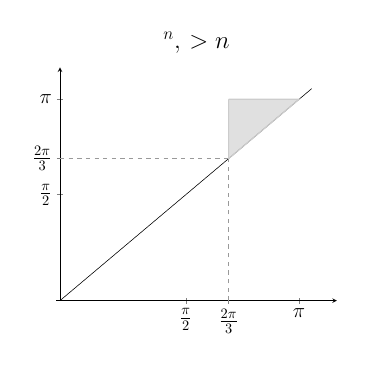
\begin{tikzpicture}[scale=0.52]
	\begin{axis} [
		title={\LARGE $\Hbarc{\degp}{\rp^n},\, \degp>n$},
		ticklabel style = {font=\Large},
		axis y line=middle,
		axis x line=middle,
		ytick={0.5,0.67,0.95},
		yticklabels={$\frac{\pi}{2}$,$\frac{2\pi}{3}$,$\pi$},
		xtick={0.5,0.67,0.95},
		xticklabels={$\frac{\pi}{2}$,$\frac{2\pi}{3}$,$\pi$},
		xmin=-0.015, xmax=1.1,
		ymin=0, ymax=1.1,]
		\addplot [mark=none] coordinates {(0,0) (1,1)};
		\addplot [thick,color=black!20!white,fill=black!30!white,
		fill opacity=0.4]coordinates {
			(0.67,0.95)
			(0.67,0.67)
			(0.95,0.95)
			(0.67,0.95)};
		\addplot [black!40!white,mark=none,dashed, thin] coordinates {(0,0.67) (0.67,0.67)};
		\addplot [black!40!white,mark=none,dashed, thin] coordinates {(0.67,0) (0.67,0.67)};
		% \addplot[barccolor,mark=*] (0, 0.67) circle (2pt) node[above right,barccolor]{\Large\textsf{1}};
		% \node[mark=none] at (axis cs:0.68,0.21){$\Hbarc{\degp}{\rp^n},\, \degp\geq 2$};
	\end{axis}
\end{tikzpicture}

\begin{tikzpicture}[scale=0.52]
	\begin{axis} [
		title = {\LARGE $\sqbarcl{k}{}{\rp^n},\, m \leq n$ and $\binom{m-k}{k}$ odd},
		ticklabel style = {font=\Large},
		axis y line=middle,
		axis x line=middle,
		ytick={0.5,0.67,0.95},
		yticklabels={$\frac{\pi}{2}$,$\frac{2\pi}{3}$,$\pi$},
		xtick={0.5,0.67,0.95},
		xticklabels={$\frac{\pi}{2}$,$\frac{2\pi}{3}$,$\pi$},
		xmin=-0.015, xmax=1.1,
		ymin=0, ymax=1.1,]
		\addplot [mark=none] coordinates {(0,0) (1,1)};
		\addplot [thick,color=black!20!white,fill=black!30!white,
		fill opacity=0.4]coordinates {
			(0.67,0.95)
			(0.67,0.67)
			(0.95,0.95)
			(0.67,0.95)};
		\addplot [black!40!white,mark=none,dashed, thin] coordinates {(0,0.67) (0.67,0.67)};
		%\addplot [black!40!white,mark=none,dashed, thin] coordinates {(0,0.72) (0.72,0.72)};
		\addplot [black!40!white,mark=none,dashed, thin] coordinates {(0.67,0) (0.67,0.67)};
		\addplot[barccolor,mark=*] (0, 0.67) circle (2pt) node[above right,barccolor]{};
        %{\Large$\geq$\textsf{1}};
	\end{axis}
\end{tikzpicture}
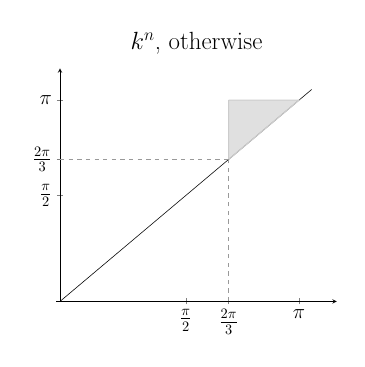
\begin{tikzpicture}[scale=0.52]
	\begin{axis} [
		title={\LARGE $\sqbarcl{k}{}{\rp^n}$, otherwise},
		ticklabel style = {font=\Large},
		axis y line=middle,
		axis x line=middle,
		ytick={0.5,0.67,0.95},
		yticklabels={$\frac{\pi}{2}$,$\frac{2\pi}{3}$,$\pi$},
		xtick={0.5,0.67,0.95},
		xticklabels={$\frac{\pi}{2}$,$\frac{2\pi}{3}$,$\pi$},
		xmin=-0.015, xmax=1.1,
		ymin=0, ymax=1.1,]
		\addplot [mark=none] coordinates {(0,0) (1,1)};
		\addplot [thick,color=black!20!white,fill=black!30!white,
		fill opacity=0.4]coordinates {
			(0.67,0.95)
			(0.67,0.67)
			(0.95,0.95)
			(0.67,0.95)};
		\addplot [black!40!white,mark=none,dashed, thin] coordinates {(0,0.67) (0.67,0.67)};
		\addplot [black!40!white,mark=none,dashed, thin] coordinates {(0.67,0) (0.67,0.67)};
	\end{axis}
\end{tikzpicture}
	\caption{\emph{Top row:} usual barcodes of $\rp^n$. \emph{Bottom row:} Steenrod barcodes of $\rp^n$. See \cref{subsub:general_barcodes}.}
	\label{fig:sq barcodes}
\end{figure}

\subsection{First critical values}

We first identify some important quantities, referred to as first critical values, that will help us estimate the barcodes.

\subsubsection{}
\label{subsub:first_critical_value}

% Let $\cX$ be an $n$-dimensional manifold.
 Let $X$ be an $\R$-space which is empty for negative numbers.
Its \defn{first critical value} is the supremum among real numbers $r$ such that $X_{s,t}$ is a homotopy equivalence for any $s,t \in [0,r]$. 

Let $V$ be a persistence module which is $0$ for negative numbers.
Its \defn{first critical value} is defined similarly. 

\medskip\example
By \cref{prop:homotopy type}, the first critical value $\VR(\rp^n)$ is $\tfrac{2\pi}{3}$.

The first critical value $\beta_\degp$ of the $\degp$-th homology of $\VR(\rp^n)$ is $\tfrac{2\pi}{3}$, for any $1 \leq \degp \leq n$. We will prove this as the lemma in \cref{subsub:foundamental_bar_rpn}.
    

\medskip\lemma
For positive integers such that $k \leq \min\{\frac{n-1}{2}, \ell\} \leq n$ and $\binom{\ell}{k}$ odd,
the first critical value $\gamma_{k+\ell}$ of $\img (\Sq^k \colon \rH^\ell(\rp^n) \to \rH^{\ell+k}(\rp^n))$ is $\tfrac{2\pi}{3}$.

\begin{proof}
	Assuming $k$ and $\ell$ satisfy the required conditions.
	Since the Vietoris--Rips complex $\VR_r(\rp^n)$ retains the homotopy type of $\rp^n$ for $r \in (0,\tfrac{2\pi}{3})$, $\Sq^k(\alpha^\ell) = \binom{\ell}{k}\alpha^{\ell+k}$ generates a bar in the $\Sq^k_\ell$--barcode that is born at $0$ and stay alive until the non-trivial degree-$(\ell+k)$ class $\alpha^{k+\ell}$ dies at $\tfrac{2\pi}{3}$.
        Thus, the first critical value of $\gamma_{k+\ell} \leq \tfrac{2\pi}{3}$.
        On the other hand, $\gamma_{k+\ell} \geq \alpha = \tfrac{2\pi}{3}$ the first critical value of $\VR(\rp^n)$.
        Thus, $\gamma_{k+\ell} = \tfrac{2\pi}{3}$.
\end{proof}

\ling{reminder: move the remark below to be before the lemma.}

\medskip\remark
Clearly, the first critical value of an $\R$-space is bounded above by the first critical value of its $m$-homology, as well as that of any 
For general spaces, these first critical values are not necessarily the same, but we always have $\alpha \leq \beta_m$ and $\alpha \leq \gamma_m$.

% We show that for any degree $1 \leq \degp \leq n$, the first critical value of the $\degp$-th homology of the Vietoris-Rips filtration of $\rp^n$ is $\tfrac{2\pi}{3}.$

\subsubsection{}

\ling{We need to be careful with the citation here: (1) cite \cite{adams2022metric} for the original definition; (2) cite Liam Barham for the fixed definition. 
We should ask Liam Barham for permission to cite his unpublished work.}

Let $G$ be a group acting properly and by isometries on a metric space $\cX$.
Let $r_0>0$. The action of a group $G$ on $\cX$ is an \defn{$r_0^*$-diameter action} if for any non-negative integer $k$, $\diam_{\cX_G}\{[x_0],\dots,[x_k]\}<r_0$ implies that there exist unique choice of $g_i$'s for $1\leq i\leq k$ such that $\diam_{\cX}\{x_0,g_1x_1,\dots,g_kx_k\}<r_0$. 

Assume the action of $G$ on $\cX$ is a $r_0^*$-diameter action for some $r_0> 0$.
In \cite[Proposition 3.5]{adams2022metric}, the authors constructed a homeomorphism from $\VR_r^m(\cX_G)$ to $\VR_r^m(\cX)_G$ for all $r \leq r_0$.
We review their constructions below. 

Define the map $h$ to be
\[
h \colon \VR_r^m(\cX) \to \VR_r^m(\cX_G) 
\text{ with }
\sum_{i=1}^k \lambda_i x_i \mapsto \sum_{i=1}^k \lambda_i [x_i],
\]
Because $G$ acts isometrically, $h$ is well-defined.
Because two points in the same orbit of the $G$ action always have the same image under $h$, it induces a map $h_G \colon \VR_r^m(\cX)_G \to \VR_r^m(\cX_G)$.
Moreover, $h_G$ is an isomorphism, following from the fact that the action of $G$ on $\cX$ is an $r^*$-diameter action; see \cite[Proposition 3.5]{adams2022metric} for further details.

Assuming that the action of $G$ on $\cX$ is a $r_0^*$-diameter action, for any $0<r<r_0$, we can consider the inverse of $h_G$ and we denote it as
\[
h \colon \VR_r^m(\cX_G) \to \VR_r^m(\cX)_G
\text{ with }
\sum_{i=1}^k \lambda_i [x_i] \mapsto [\sum_{i=1}^k \lambda_i x_i].
\]


\subsubsection{}

Let $\bS^n$ the sphere of radius $2$ and let $G=\Z/2\Z$ act on $\bS^n$ by identifying the antipodal points.
It follows from \cite[Corollary]{adams2022metric} that the action of $G$ on $\bS^n$ is a $r^*$-diameter action for any $r<\tfrac{2\pi}{3}$.

For any $r<\pi$, let $\tilde{f}^n$ be the composition
\[
    \tilde{f}^n \colon \VR_r^m(\bS^n) \to \R^{n+1} \setminus \set{0} \xra{\pi^n} \bS^n,
\]
where the first map sends a formal linear sum $\sum_{i=1}^k \lambda_i x_i$ in the Vietoris--Rips thickening $\VR_r^m(\bS^n)$ to the point $\sum_{i=1}^k \lambda_i x_i \in \bbR^{n+1}$ where $x_i \in \bS^n$ and $\lambda_i \in [0,1]$ satisfying $\sum_i\lambda_i=1$, and the second map $\pi^n$ is the radial projection map.

By \cite[Proposition 5.3]{adamaszek2018metric}, the map $\tilde{f}^n$ is a homotopy equivalence for all $0<r<\zeta_n=\arccos{(-\tfrac{1}{n+1})}$.
% When $n=1$, this is $\tfrac{4\pi}{3}.$

Because $\tilde{f}^n$ preserves group action, i.e. $\tilde{f}^n(x) = \tilde{f}^n(gx)$ for any $x\in \bS^n$ and $g\in G$, we have the homotopy equivalence for $0<r<\zeta_n$, %\anibal{Maybe use superscripts for these maps and the $\rho$ too?}
\[
\tilde{f}^n_G \colon 
\VR_r^m(\bS^n)_G \, 
\to \bS^n_G.
%\cong \rp^n.
\]
By composing $h^n$ with $\tilde{f}^n_G$, we obtain a map 
\[
\rho^n = h^n \circ \tilde{f}^n_G 
\colon \VR_r^m(\bS^n_G) \to \bS^n_G
\]

\subsubsection{} 

For $0<t\leq s \leq s'$, we consider the following diagram of topological spaces:
\begin{equation}\label{d:fundamental_bars_diagram}
    \begin{tikzcd}
        \bS^{n-1}_G
        \ar[d, hook,"{\iota}" left]
        &
        \VR_t(\bS^{n-1}_G)
        \ar[d, hook,"\iota_r"]
        \ar[l, "\rho^{n-1}" above, "\simeq" below]
        \ar[r, hook, "v^{n-1}"]
        &
        \VR_{s}(\bS^{n-1}_G)
        \ar[d, hook]
        \\
        \bS^{n}_G
        &
        \VR_t(\bS^{n}_G)
        \ar[l, "\rho^n" below, "\simeq" above]
        \ar[r, hook, "v^{n}"]
        &
        \VR_{s'}(\bS^{n}_G).
    \end{tikzcd}
\end{equation}
Here, the horizontal inclusions $v^{n-1}$ and $v^n$ are induced by the Vietoris--Rips filtration, whereas the vertical maps are induced by the equatorial inclusion of real projective spaces $\iota \colon \bS^{n-1}_G \hookrightarrow \bS^{n}_G$.

We claim that diagram \eqref{d:fundamental_bars_diagram} commutes. 
The commutativity of the right-hand-side square is straightforward.
For the left-hand-side square, we need to verify that $\iota \circ \rho^{n-1}=\rho^{n} \circ \iota_r$.
\ling{notation for maps below need to be fixed at the end.}
Indeed, for any $y = \sum_{i=1}^k \lambda_i [x_i] \in \VR_t(\bS^{n-1}_G)$, we have
\begin{center}
    $(\iota \circ \rho^{n-1})(y)
    =\iota(f^{n-1}/\sim([\sum_i \lambda_i x_i]))
    =\iota([f^{n-1}(\sum_i \lambda_i x_i)])
    =[\pi^{n-1}(\sum_i \lambda_i x_i)]
    $
\end{center}
as an element in $\bS^n_G$, and
\begin{center}
    $(\rho^{n} \circ \iota_r)(y) = \rho^{n}(y) = f^{n}/\sim([\sum_i \lambda_i x_i]) = [f^{n}(\sum_{i=1}^k \lambda_i x_i)] = [\pi^{n}(\sum_{i=1}^k \lambda_i x_i)]
    $
\end{center}
Because $\pi^{n}$ restricted to $\bS^{n-1}_G$ is equal to $\pi^{n-1}$, we conclude that $(\iota \circ \rho^{n-1})(y) = (\rho^n \circ \iota_r)(y)$ for any $y$.
Thus, the claim holds.

\subsubsection{}
\label{subsub:foundamental_bar_rpn}

Let $\delta_n=2\fillrad[\field]{\bS^n_G}$ and 
let $\alpha_1$ be the first critical value of $\VR(\bS^1_G)$.
For any degree $1 \leq \degp \leq n$, let $\beta_{\degp, n}$ be the first critical value of the $\degp$-th homology of $\VR(\bS^n_G)$. 

\medskip\lemma 
If $\delta_1 = \dots = \delta_n \leq \alpha_1$ and $\beta_{\degp, n} \leq \beta_{\degp, n'}$ for any $n\leq n'$, then
\[
\beta_{m, n} = \delta_1, \, \text{for any $1 \leq m \leq n$.}
\]

\begin{proof}
	We will use an induction argument on $n$.
	When $n = 1$, it follows from the lemma in \cref{ss:filling_radius} that
	\[
	(0, 2\fillrad[\field]{\bS^1_G}) = (0, \delta_1) \in \Hbarc[\field]{1}{\bS^1_G}.
	\]
        This implies that $\rH_1(\VR(\bS^1_G))$ changes isomorphism types at $\delta_1$, so $\beta_{1, 1} \leq \delta_1$.
        On the other hand, because $\delta_1 \leq \alpha_1$, $\rH_1(\VR(\bS^1_G))$ retains the same isomorphism type before $\delta_1$, implying that $\beta_{1, 1} \geq \delta_1$.
        Thus, $\beta_{1, 1} =\delta_1$. 
        
	Assume the statement holds for $\bS^{n-1}_G$, that is, $\beta_{m, n-1} = \delta_1$ for any $1\leq m \leq n-1$.
    Applying the $\degp$-th homology functor to diagram \eqref{d:fundamental_bars_diagram}, we obtain the following commutative diagram of vector spaces:
    for $r,\epsilon>0$ small,
    \[
    \begin{tikzcd}
        \rH_\degp(\bS^{n-1}_G)
        \ar[d, "\cong" left]
        &
        \rH_\degp(\VR_r(\bS^{n-1}_G))
        \ar[d, "\rH_\degp(\iota_r)" left, "\cong" right, myred]
        \ar[l, "\cong" above]
        \ar[rr, "\rH_\degp(v^{n-1})=0", myred]
        &
        &
        \rH_\degp(\VR_{\delta_1+\epsilon}(\bS^{n-1}_G))
        \ar[d]
        \\
        \rH_\degp(\bS^{n}_G)
        &
        \rH_\degp(\VR_r(\bS^{n}_G))
        \ar[l, "\cong"]
        \ar[rr, "\rH_\degp(v^n)" , myred]
        &
        &
        \rH_\degp(\VR_{\delta_1+\epsilon}(\bS^{n}_G)).
    \end{tikzcd}
    \]
    Here, $\rH_\degp(f)$ for some map $f$ between topological spaces denotes the induced map of $f$ on the $\degp$-th homology. 

    Commutativity of the left-hand-side square implies that $\rH_\degp(\iota_r)$ is an isomorphism.
    By induction assumption, $\beta_{m, n-1} = \delta_1$ is the first critical value of $\rH_\degp(\VR(\bS^{n-1}_G))$, which implies that $\rH_\degp(v^{n-1})$ is the zero map.
    Then, using the right-hand-side square's commutativity, we deduce $\rH_\degp(v^n) \circ \rH_\degp(\iota_r)=0$.
    Since $\rH_\degp(\iota_r)$ is an isomorphism, we conclude that $\rH_\degp(v^n)=0$.
    This holds for any $\epsilon>0$, so we can conclude $\beta_{m, n} \leq \delta_1$. 
    On the other hand, we have $\delta_1 = \beta_{m, n-1} \leq \beta_{m, n}$. 
    Therefore, $\beta_{m, n} = \delta_1$ holds for any $1\leq m \leq n-1$.
	
	For the case when $\degp=n$, we can apply the lemma in \textsection \ref{ss:filling_radius} to obtain 
    \[
    (0,2\fillrad{\bS^n_G}) = (0, \delta_n) = (0, \delta_1) \in \Hbarc{n}{\bS^n_G}.
    \]
        
	Therefore, $(0, \delta_1) \in \Hbarc[\field]{\degp}{\bS^n_G}$ is established for all $1\leq \degp\leq n.$
\end{proof}

We will refer to the bar in this lemma as the \defn{fundamental bar} of $\bS^n_G$.

\example Recall that the filling radius of $\rp^n$ is $\frac{\pi}{3}$ for any $n \geq 1$.
Therefore, \cref{ss:filling_radius} gives that $\delta_n = \tfrac{2\pi}{3} = \alpha_1$ for all $n$.
Additionally, we have that
\[
\rp^1 \subset \rp^2 \subset \dots \subset \rp^n,
\]
with $\rp^\degp$ generating the $\degp^\th$ mod 2 homology of $\rp^n$ for every $1 \leq \degp \leq n$.
This implies that $\beta_{\degp, n} \leq \beta_{\degp, n'}$ for any $n\leq n'$ and $m$.
Applying the above lemma, we obtain $\beta_{m,n} = \delta_1 = \tfrac{2\pi}{3},$ for any $n\geq 1$ and $1 \leq m \leq n$.

\subsection{Barcode estimates}
\label{subsub:general_barcodes}

Let $\cX$ be an $n$-dimensional manifold with diameter $\pi$ such that the first critical value of $\VR(\cX)$ is greater than $\zeta_n$.
From now on, we will consider this $\R$-space and omit it from the notation.
% \begin{itemize}
%     \item $\mathrm{H}_\degp (\cX; \field)\cong \field$ for any $1\leq \degp\leq n$ and some field $\field$.\anibal{I would not impose this}
    
%     %\item the first critical value of the $\degp$-th homology of $\VR(\cX)$ is less than $\tfrac{\zeta_n}{2}+\zeta_\degp .$
% \end{itemize}

Let $\theta \in \cO(\ell, \degp; \kk)$ be a linear cohomology operation with $1 \leq \ell, \degp \leq n$. 
%$\theta_\cX \colon \rH^n(\cX; \pi) \to \rH^m(\cX; G)$.
Let $\beta_\degp$ and $\gamma_\degp$ be the first critical values of $\rH_\degp$ and $\img \theta$, respectively.
Then we have the following estimates of the usual barcodes and the $\theta$-barcodes of $\cX$. 
\begin{itemize}
    \item The usual barcodes of $\cX$ satisfy the following properties:
        \begin{itemize}
            \item For any $1 \leq \degp \leq n$, $\Hbarc[\field]{\degp}{\cX}$ contains $(0,\beta_\degp )$ for some $\beta_\degp \in [\alpha, \pi)$ and possibly some bars dominated by $(\alpha, \pi)$.
            \item For $\degp > n$, all bars in $\Hbarc[\field]{\degp}{\cX}$ are dominated by $(\alpha, \pi)$.
        \end{itemize}
    \item The $\theta$-barcodes of $\cX$ satisfy the following properties: 
        \begin{itemize}
            \item For $1 \leq \degp \leq n$ such that the image of $\theta_\cX \colon \rH^\ell(\cX; \field) \to \rH^\degp(\cX; \field)$ is non-trivial, $\thetabarc{\cX}$ contains at least one bar $(0,\gamma_\degp )$ for some $\gamma_\degp \in [\alpha, \pi)$ and possibly some bars dominated by $(\alpha, \pi)$. 
            \item For $\degp$ such that $\img \theta_\cX$ is trivial, all bars in $\thetabarc{\cX}$ are dominated by $(\alpha, \pi)$. 
        \end{itemize}
\end{itemize}

\example 
In the case of the real projective planes and Steenrod squares, we have seen in \cref{subsub:first_critical_value} that $\alpha = \beta_\degp = \gamma_{k+\ell} = \tfrac{2\pi}{3}$ for any $1 \leq \degp \leq n$ and $k, \ell$ such that $k \leq \frac{n-1}{2}$ s.t. $\binom{\ell}{k} \mod 2\neq 0$. 
By plugging in these values to the above discussion, we obtain an estimate of the barcodes of $\rp^n$, as illustrated in \cref{fig:sq barcodes}.

%\subsubsection{}\label{prop:RPn bar}

% \medskip\lemma For integers $1 \leq \degp \leq n$ we have
% \[
% \left(0, \tfrac{2\pi}{3}\right) \in \Hbarc{\degp}{\rp^n}.
% \]

% \begin{proof}
% 	We will use an induction argument on $n$.
% 	When $n = 1$, \cref{ss:filling_radius} implies that
% 	\[
% 	(0, 2\fillrad{\rp^1}) = \left(0, \tfrac{2\pi}{3}\right) \in \Hbarc{1}{\rp^1}.
% 	\]
% 	Assume the statement holds for $\rp^{n-1}$.
% 	That is, for any $1 \leq \degp \leq n-1$,
% 	\[
% 	\left(0, \tfrac{2\pi}{3}\right) \in \Hbarc{\degp}{\rp^{n-1}}.
% 	\]
% 	Let $r, \epsilon > 0$ be small.
% 	We claim that the following diagram of topological spaces commutes:
% 	\begin{equation}\label{d:fundamental_bars_diagram}
% 		\begin{tikzcd}
% 			\rp^{n-1}
% 			\ar[d, hook,"{\iota}" left]
% 			&
% 			\VR_t(\rp^{n-1})
% 			\ar[d, hook,"\iota_t"]
% 			\ar[l, "\rho^{n-1}" above, "\simeq" below]
% 			\ar[r, hook]
% 			&
% 			\VR_{\tfrac{2\pi}{3}+\epsilon}(\rp^{n-1})
% 			\ar[d, hook]
% 			\\
% 			\rp^{n}
% 			&
% 			\VR_t(\rp^{n})
% 			\ar[l, "\rho^n" below, "\simeq" above]
% 			\ar[r, hook]
% 			&
% 			\VR_{\tfrac{2\pi}{3}+\epsilon}(\rp^{n}).
% 		\end{tikzcd}
% 	\end{equation}
% 	In the above diagram, the horizontal inclusions are induced by the Vietoris--Rips filtration, whereas the vertical maps are induced by the equatorial inclusion of real projective spaces $\iota \colon \rp^{n-1} \hookrightarrow \rp^{n}$.
% 	It is therefore clear that the right square of \eqref{d:fundamental_bars_diagram} commutes.
	
% 	We now construct the remaining two maps $\rho^{n-1}$ and $\rho^{n}$ as in \cite[\textsection 4.3]{adams2022metric}.
% 	Let $f^n$ be the composition
% 	\[
% 	f^n \colon \VR_t(\bS^n) \to \R^{n+1} \setminus \set{0} \xra{\pi^n} \bS^{n},
% 	\]
% 	where the first map sends a formal linear sum $\sum_{i=1}^k \lambda_i x_i$ in $\VR_t(\bS^n)$ to the sum $\sum_{i=1}^k \lambda_i x_i \in \bbR^{n+1}$ where $x_i \in \bS^{n}$ and $\lambda_i \in \bbR$, and the second map $\pi^n$ is the radial projection map.
% 	Because $f^n$ preserves the equivalence relation $x \sim -x$, we have the induced map %\anibal{Maybe use superscripts for these maps and the $\rho$ too?}
% 	\[
% 	f^n/\sim \colon \VR_t(\bS^{n})/\sim\to \bS^{n}/\sim\cong \rp^n.
% 	\]
% 	Because $r < \tfrac{2\pi}{3}$, it follows from \cite[Lemma 4.4]{adams2022metric} that the map
% 	\[
% 	\alpha^n \colon \VR_t(\rp^n) \to \VR_t(\bS^n)/\sim \text{ with }
% 	\sum_{i=1}^k \lambda_i [x_i] \mapsto \left[\sum_{i=1}^k \lambda_i x_i\right]
% 	\]
% 	is a homeomorphism, where $x_i \in \bS^{n}$, $\lambda_i \in \bbR$, and $[\cdot]$ denotes the equivalence class of an element under the relation $x \sim -x$. \ling{check if $\sum \lambda_i = 1$.}
% 	We define
% 	\[\rho^n = \alpha^n \circ f^n/\sim \]
% 	It is shown in \cite[Theorem 4.5]{adams2022metric} that $\rho^n$ is a homotopy equivalence from $\VR_t(\rp^n)$ to $\rp^n$ for any $n$.
% 	% In summary, we have defined the map
% 	% \[\rho^n: \VR_t(\rp^n)\xrightarrow{\cong} \VR_t(\bS^n)/\sim\to \bS^{n}/\sim\cong \rp^n\]
	
% 	We claim that the left square in the previous diagram commutes, i.e. $\iota \circ \rho^{n-1}=\rho^{n} \circ \iota_t$.
% 	Indeed, for any $y = \sum_{i=1}^k \lambda_i [x_i] \in \VR_t(\rp^{n-1})$, we have
% 	\begin{center}
% 		$(\iota \circ \rho^{n-1})(y)
% 		=\iota(f^{n-1}/\sim([\sum_i \lambda_i x_i]))
% 		=\iota([f^{n-1}(\sum_i \lambda_i x_i)])
% 		=[\pi^{n-1}(\sum_i \lambda_i x_i)]
% 		$
% 	\end{center}
% 	as an element in $\rp^n$, and
% 	\begin{center}
% 		$(\rho^{n} \circ \iota_t)(y) = \rho^{n}(y) = f^{n}/\sim([\sum_i \lambda_i x_i]) = [f^{n}(\sum_{i=1}^k \lambda_i x_i)] = [\pi^{n}(\sum_{i=1}^k \lambda_i x_i)]
% 		$
% 	\end{center}
% 	Because $\pi^{n}$ restricted to $\rp^{n-1}$ is equal to $\pi^{n-1}$, we conclude that $(\iota \circ \rho^{n-1})(y) = (\rho^n \circ \iota_t)(y)$ for any $y$.
% 	Thus, the claim holds.
	
% 	For each $1 \leq \degp \leq n-1$, applying the $\degp$-th homology functor (over $\Ftwo$) to the above diagram, we obtain the following commutative diagram of vector spaces:
% 	\[
% 	\begin{tikzcd}
% 		\rH_\degp (\rp^{n-1})
% 		\ar[d, "\cong" left]
% 		&
% 		\rH_\degp (\VR_t(\rp^{n-1}))
% 		\ar[d, "\rH_\degp (\iota_t)" left, "\cong" right, myred]
% 		\ar[l, "\cong" above]
% 		\ar[r, "g^{n-1}=0", myred]
% 		&
% 		\rH_\degp (\VR_{\tfrac{2\pi}{3}+\epsilon}(\rp^{n-1}))
% 		\ar[d]
% 		\\
% 		\rH_\degp (\rp^{n})
% 		&
% 		\rH_\degp (\VR_t(\rp^{n}))
% 		\ar[l, "\cong"]
% 		\ar[r, "g^n" , myred]
% 		&
% 		\rH_\degp (\VR_{\tfrac{2\pi}{3}+\epsilon}(\rp^{n})).
% 	\end{tikzcd}
% 	\]
% 	By induction assumption, $(0, \tfrac{2\pi}{3})\in\Hbarc{\degp}{\rp^{n-1}}$, which implies that $g^{n-1}$ is the zero map.
% 	Commutativity of the left-hand side square further implies that $\rH_\degp (\iota_t)$ is an isomorphism.
% 	Then, using the right-hand side square's commutativity, we deduce $g^n \circ \rH_\degp (\iota_t)=0$.
% 	Since $\rH_\degp (\iota_t)$ is an isomorphism, we conclude that $g^n=0$.
% 	This holds for any $\epsilon>0$, so we can conclude $(0, \tfrac{2\pi}{3})\in\Hbarc{\degp}{\rp^{n}}$.
	
% 	For the case when $m=n$, we can apply Item (\ref{ss:filling_radius}) to observe that $(0,2\fillrad{\rp^n}) = (0, \tfrac{2\pi}{3}) \in \Hbarc{n}{\rp^n}$.
% 	Therefore, $(0, \tfrac{2\pi}{3}) \in \Hbarc{\degp}{\rp^n}$ is established for all $1 \leq \degp \leq n.$
% \end{proof}

% We will refer to the bar in this lemma as the \defn{fundamental bar} of $\rp^n$.

\section{Gromov--Hausdorff estimates}\label{prop:db estimate}

We estimate the bottleneck distance $\db$ between the Steenrod barcodes of the two space $\VS^n$ and $\rp^n$, and show that it provides a better (lower-bound) approximation of the Gromov--Hausdorff distance $\dgh(\VS^n, \rp^n)$ than $\db$ between the standard barcodes.
See the theorem in \cref{subsub:main_theorem} for details.
Although this theorem is stated for $\VS^n$ and $\rp^n$ only, we present our methodology within a more general framework.
This allows us to identify the essential components of the proof, laying the groundwork for extending these results to other spaces.

\subsection{Upper bound on $\db$ between usual barcodes}
\label{subsub:db_upper_bound}

To obtain an upper bound on the bottleneck distance, it suffices to find one matching and compute the cost of it. 

For any degree $1 \leq \degp \leq n$, consider the matching $P$ between $\Hbarc[\field]{\degp}{\VS}$ and $\Hbarc[\field]{\degp}{\cX}$ such that $(0,\zeta_\degp ) \leftrightarrow (0, \beta_\degp )$ and all other bars unmatched. 
Then the cost of $P$ satisfies
\begin{align*}
    \cost(P) 
    = & \max\{|\zeta_\degp  - \beta_\degp |, \tfrac{\pi - \zeta_n}{2}, \tfrac{\pi - \alpha}{2}\} \\
    = & \max\{|\zeta_\degp  - \beta_\degp |, \tfrac{\pi - \zeta_n}{2}\} && \mbox{(because $\zeta_n \leq \alpha$)}.
\end{align*}

Therefore, for any degree $1 \leq \degp \leq n$,
\begin{equation}\label{eq:db_usual_upper_bound}
    \db(\Hbarc[\field]{\degp}{\VS^n}, \Hbarc[\field]{\degp}{\cX})
    \leq \cost(P) 
    = \max\{|\zeta_\degp  - \beta_\degp |, \tfrac{\pi - \zeta_n}{2}\}.
\end{equation}

% For any degree $m > n$, consider the matching $m$ between $\Hbarc[\field]{\degp}{\VS}$ and $\Hbarc{\degp}{\cX}$ such that all bars are unmatched. Then the cost of $m$ satisfies:
% \[
%     \cost(P) 
%     = \max\{\tfrac{\pi - \zeta_n}{2}, \tfrac{\pi - \alpha}{2}\} 
%     = \tfrac{\pi - \zeta_n}{2}. 
% \]

\subsection{Lower bound on $\db$ between $\theta$-barcodes}
\label{subsub:db_theta_lower_bound}

To obtain a lower bound on the bottleneck distance, the minimum cost of matching a certain bar is calculated. 

Let $\theta \in \cO(\ell, \degp; \kk)$, for some $1 \leq \ell, \degp \leq n$, be a linear cohomology operation such that $\img \theta_\cX$ is non-trivial.
We calculate the minimum cost of matching the bar $(0,\gamma_\degp )$ in $\thetabarc{\cX}$.

Let $Q$ be an arbitrary matching between $\thetabarc{\VS}$ and $\thetabarc{\cX}$.
If $(0,\gamma_\degp )$ is unmatched in $Q$, then $\cost(Q) \geq \tfrac{\gamma_\degp }{2}$. 
If $(0,\gamma_\degp )$ is matched to some bar $(a,b) \in \thetabarc{\VS}$ in $Q$, then 
$\cost(Q) =  \|(0,\gamma_\degp ) - (a,b)\|_\infty \geq  a \geq \alpha \geq \zeta_n$.
Thus, an arbitrary matching $Q$ between $\thetabarc{\VS}$ and $\thetabarc{\cX}$ must satisfy $\cost(Q) 
    \geq \min\{\tfrac{\gamma_\degp }{2}, \zeta_n\}.$
    
Therefore, 
\begin{equation}\label{eq:db_theta_lower_bound}
    \db(\thetabarc{\VS^n}, \thetabarc{\cX})
    = \min_Q \cost(Q) 
    \geq \min\{\tfrac{\gamma_\degp }{2}, \zeta_n\}. %\geq \tfrac{\zeta_n}{2}.
\end{equation}

\subsection{Technical lemma}
\label{subsub:comparison_lemma}

We establish a technical lemma.  

\medskip\lemma 
\begin{itemize}
    \item If $\beta_\degp \in [\alpha, \tfrac{\pi - \zeta_n}{2}+\zeta_\degp]$, then
            $\max\{|\zeta_\degp  - \beta_\degp |, \tfrac{\pi - \zeta_n}{2}\}
            \leq \tfrac{\pi - \zeta_n}{2}$.
    \item If $\beta_\degp \in (\tfrac{\pi - \zeta_n}{2}+\zeta_\degp, \tfrac{\zeta_n}{2}+\zeta_\degp)$, then
            $\max\{|\zeta_\degp  - \beta_\degp |, \tfrac{\pi - \zeta_n}{2}\}
            \leq \tfrac{\zeta_n}{2}$.
\end{itemize}

\begin{proof}
        First consider when $\beta_\degp \in [\alpha, \tfrac{\pi - \zeta_n}{2}+\zeta_\degp]$ and divide the discussion to two cases.  
        If $\beta_\degp \leq \zeta_\degp$, then because $\tfrac{\pi}{2} < \alpha \leq \beta_\degp \leq \zeta_\degp  \leq \tfrac{2\pi}{3}$ and $\zeta_n \leq \tfrac{2\pi}{3}$, we have
        \[
            |\zeta_\degp  - \beta_\degp | 
            = \zeta_\degp  - \beta_\degp  
            < \tfrac{2\pi}{3} - \tfrac{\pi}{2} 
            = \tfrac{\pi}{6} 
            \leq \tfrac{\pi - \zeta_n}{2}.
        \]
        If $\beta_\degp > \zeta_\degp$, then 
        \[
            |\zeta_\degp  - \beta_\degp | 
            = \beta_\degp - \zeta_\degp
            \leq \tfrac{\pi - \zeta_n}{2} + \zeta_\degp - \zeta_\degp 
            = \tfrac{\pi - \zeta_n}{2}.
        \]
        Thus, $\max\{|\zeta_\degp  - \beta_\degp |, \tfrac{\pi - \zeta_n}{2}\} = \tfrac{\pi - \zeta_n}{2}.$
        
        When $\beta_\degp \in (\tfrac{\pi - \zeta_n}{2}+\zeta_\degp, \tfrac{\zeta_n}{2}+\zeta_\degp)$, we have
        \[
            \max\{|\zeta_\degp  - \beta_\degp |, \tfrac{\pi - \zeta_n}{2}\}
            = \max\{\beta_\degp - \zeta_\degp, \tfrac{\pi - \zeta_n}{2}\}
            < \max\{\tfrac{\zeta_n}{2}+\zeta_\degp - \zeta_\degp, \tfrac{\pi - \zeta_n}{2}\}
            = \tfrac{\zeta_n}{2} .
        \]
\end{proof}

\subsection{Comparison}
\label{subsub:main_theorem}

By combining results from \cref{subsub:db_upper_bound}, \cref{subsub:db_theta_lower_bound} and \cref{subsub:comparison_lemma}, we immediately obtain that the lower bound of the bottleneck distance $\db$ between the $\theta$-barcodes of the two space $\VS^n$ and $\cX$ (Equation (\ref{eq:db_theta_lower_bound})) is larger than the upper bound of $\db$ between the standard barcodes of the two spaces (Equation (\ref{eq:db_usual_upper_bound})). 
As a consequence, the $\theta$-barcodes provide a better (lower-bound) approximation of the Gromov--Hausdorff distance than $\db$ between the standard barcodes.

\medskip\proposition
Let $\cX$ be an $n$-dimensional manifold with diameter $\pi$ such that
\begin{itemize}
    \item $\mathrm{H}_\degp (\cX; \field)\cong \field$ for any $1\leq \degp\leq n$ and some field $\field$.
    \item the first critical value of $\VR(\cX)$ lies in $[\zeta_n, \pi)$.
\end{itemize}
If $\theta \in \cO(\ell, \degp; \kk)$ is a linear cohomology operation such that $\img \theta_\cX$ is non-trivial, then
\[\db(\thetabarc{\VS^n}, \thetabarc{\cX}) \geq \db(\Hbarc[\field]{\degp}{\VS^n}, \Hbarc[\field]{\degp}{\cX}).\]

In the case of $\cX = \rp^n$ and the cohomology operations $\theta$ being the Steenrod squares, all with mod $2$ coefficients, we have a finer estimate as in the theorem below.

\medskip\theorem
For any $1\leq k \leq \frac{n-1}{2}$ s.t. $\binom{\ell}{k} \mod 2\neq 0$, we have
\begin{itemize} 
	\item[(a)] $\max_{\degp\geq 1}\db(\Hbarc{\degp}{\VS^n}, \Hbarc{\degp}{\rp^n})\leq \tfrac{\pi - \zeta_n}{2}$.
	\smallskip\item[(b)] $\db(\sqbarcl{k}{\ell}{\VS^n}, \sqbarcl{k}{\ell}{\rp^n})\geq \tfrac{\pi}{3}$.
\end{itemize}

\begin{proof}
        For the real-projection plane $\rp^n$, the first critical value $\alpha$ of $\VR(\rp^n)$ and the first critical value $\beta_\degp$ of the $\degp$-the homology of $\VR(\rp^n)$ are both $\tfrac{2\pi}{3}$, for any $1 \leq \degp \leq n$. %, i.e. $\alpha = \beta_\degp  = \tfrac{2\pi}{3}.$ 
        It is clear that $\alpha= \tfrac{2\pi}{3}$ lies in $[\zeta_n, \pi)$ and $\beta_\degp = \tfrac{2\pi}{3}$ lies in $[\alpha, \tfrac{\pi - \zeta_n}{2}+\zeta_\degp]$ satisfying the first condition of the above lemma. 
        Thus, the following inequality follows from \cref{eq:db_usual_upper_bound} and \cref{subsub:comparison_lemma}:
        \[\max_{\degp\geq 1}\db(\Hbarc{\degp}{\VS^n}, \Hbarc{\degp}{\rp^n})\leq \tfrac{\pi - \zeta_n}{2}.\]

        For $k \leq \frac{n-1}{2}$ s.t. $\binom{\ell}{k} \mod 2\neq 0$, we have shown in \cref{subsub:first_critical_value} that the first critical value $\gamma_{\ell+k}$ of $\sqbarcl{k}{\ell}{\rp^n}$ is $\tfrac{2\pi}{3}$. 
        Due to \cref{eq:db_theta_lower_bound}, we have
        \[\db(\sqbarcl{k}{\ell}{\VS^n}, \sqbarcl{k}{\ell}{\rp^n}) 
        \geq \min\{\tfrac{\gamma_{\ell+k}}{2}, \zeta_n\} 
        = \min\{\tfrac{1}{2}\cdot\tfrac{2\pi}{3}, \zeta_n\} 
        = \tfrac{\pi}{3}.\]
\end{proof}

Because $\tfrac{\pi}{3} < (\tfrac{\pi}{4} <) \tfrac{\pi - \zeta_n}{2}$, the above theorem shows that the Steenrod barcodes provide a better lower bound estimate of the Gromov--Hausdorff distance than the standard barcodes do in all degrees.
